%!TEX root = practicum1.tex
The parameter $K$ defines how hard the system is driven, i.e. for $K = 0$ we would expect no perturbations, this case is discussed in \cref{ss:b:trivial}. As the value of $K$ increases we expect that the chaotic regions grow and eventually start to dominate the phase space \cite{finn200Cahaotic}. The effect of varying values of $K$ is discussed in \cref{ss:b:nontrivial}. Finally \cref{ss:b:kam} discusses KAM theory and how it relates to the Chirikov map. 

\subsection{Trivial Case}
\label{ss:b:trivial}
\todo[inline]{Verwijs naar figuur \cref{fig:experiment:fancy_k:0}.}
If we choose $K = 0$ \cref{eq:chirikov} becomes:
\begin{subequations}\label{eq:chirikovK0}
	\begin{align}
		\label{eq:chirikov0:p} p_{n + 1} &= p_n \mod 1,\\
		\label{eq:chirikov0:x} x_{n + 1} &= x_n + p_{n + 1} \mod 1.
	\end{align}
\end{subequations}	
Consequently the values of $p_n$ are constant for $n > 0$, since if $p_0 = 1$, $p_1 = 0$ as a consequence of the modulo operator in \eqref{eq:chirikov0:p}. Consequently without modulo 1, $x_n$ would increase linearly, due to this operator $x_n$ is periodic. 

\Cref{fig:experiment:K0influenceOfX} shows $x_0$ as a function of $n$ for a fixed value of $p_0$, if we compare the different plots  in this figure we observe that changing $x_0$ and fixing $p_0$ only influences the phase of $x_n$, and not the period. 

\begin{figure}[t]
	\centering
	\foreach \x/\actualX in {1/0.1, 3/0.3, 5/0.5}{
		\begin{subfigure}[t]{\columnwidth}
			\includegraphics[width=\textwidth]{./img/assignment_b_K=0p_0=04x_0=0\x.pdf}
			\caption{$x_0 = \actualX$}
			\label{fig:experiment:K0:X:\x}
		\end{subfigure}	
	}	
	\caption{$x_n$ as a function of $n$, for $p_0 = 0.4$ and varying $x$.}
	\label{fig:experiment:K0influenceOfX}
\end{figure}

Fixing $x_0$ and varying $p_0$ results in \cref{fig:experiment:K0influenceOfP}, these plots show that $p_0$ influences the periodicity of the map, that is increasing $p_0$, increases the frequency.

\begin{figure}[t]
	\centering
	\foreach \p/\actualP in {1/0.1, 3/0.3, 5/0.5}{
		\begin{subfigure}[t]{\columnwidth}
			\includegraphics[width=\textwidth]{./img/assignment_b_K=0p_0=0\p x_0=04.pdf}
			\caption{$p_0 = \actualP$}
			\label{fig:experiment:K0:P:\p}
		\end{subfigure}	
	}	
	\caption{$x_n$ as a function of $n$, for $x_0 = 0.4$ and varying $p$.}
	\label{fig:experiment:K0influenceOfP}
\end{figure}

\todo[inline]{In Caption van \cref{fig:experiment:fancy_k} assen enzo beschrijven.}
\begin{figure*}
	\centering
	\foreach \k/\fnk in {0/0, 0.2/2, 0.4/4, 0.8/8, 1/10, 2/20, 3/30, 4/40}{
		\begin{subfigure}{0.32\textwidth}
			\centering
			\includegraphics[width=\textwidth]{./img/assignment_b_fancy_k_\fnk.jpg}
			\caption{$K = \k$}
			\label{fig:experiment:fancy_k:\fnk}
		\end{subfigure}
	}
	\begin{subfigure}{0.32\textwidth}
			\centering
			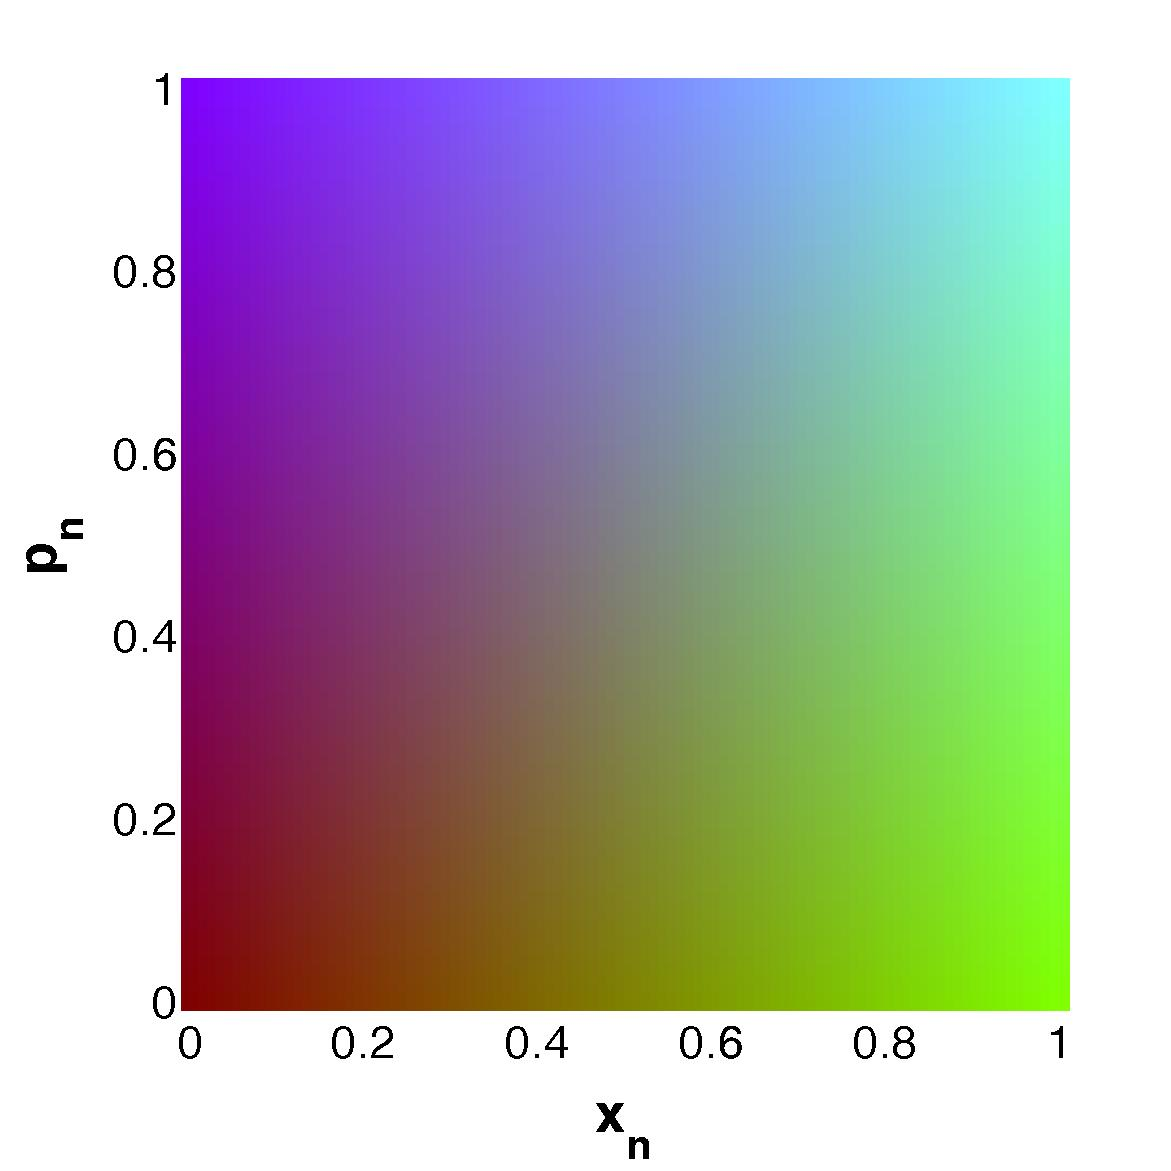
\includegraphics[width=\textwidth]{./img/assignment_b_colormap.jpg}
			\caption{Color map}
			\label{fig:experiment:fancy_k:colormap}
		\end{subfigure}
	\caption{Full 100 run chirikov maps, for different $K$. For each map 1000 iterations and random initialisation for $x_0$ and $p_0$ were used.}
	\label{fig:experiment:fancy_k}
\end{figure*}

% \begin{figure}
% 	\centering
% 	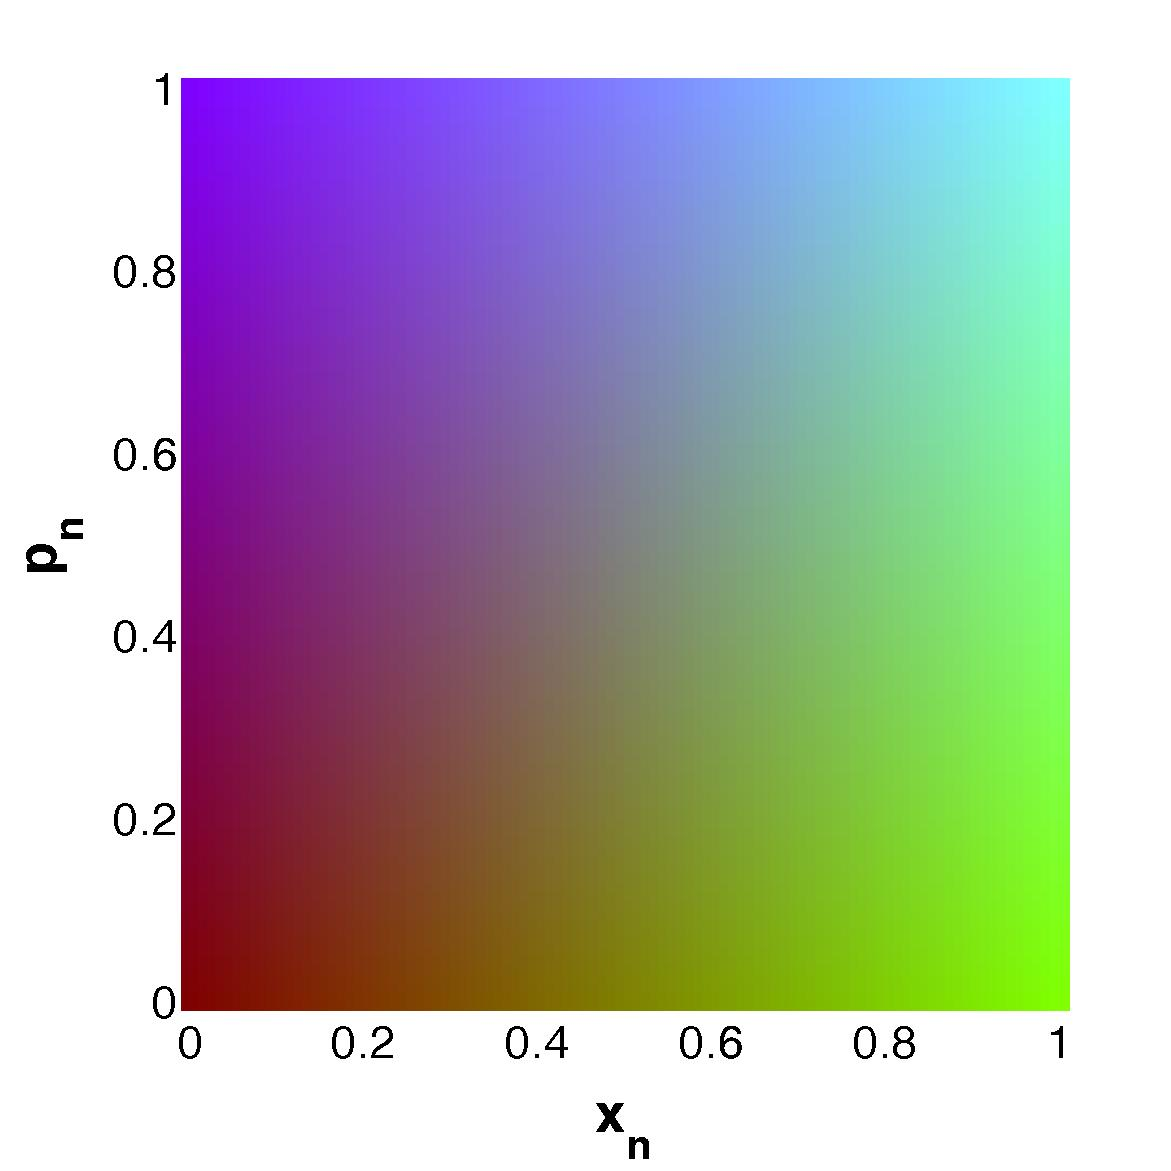
\includegraphics[width=0.6\columnwidth]{./img/assignment_b_colormap.jpg}
% 	\caption{Colour map for the colours used in \cref{fig:experiment:fancy_k} and \ref{fig:experiment:b:testKC}.}
% 	\label{fig:experiment:colormap}
% \end{figure}

\begin{figure*}[h!]
	\centering
	\begin{subfigure}{\columnwidth}
		\centering
			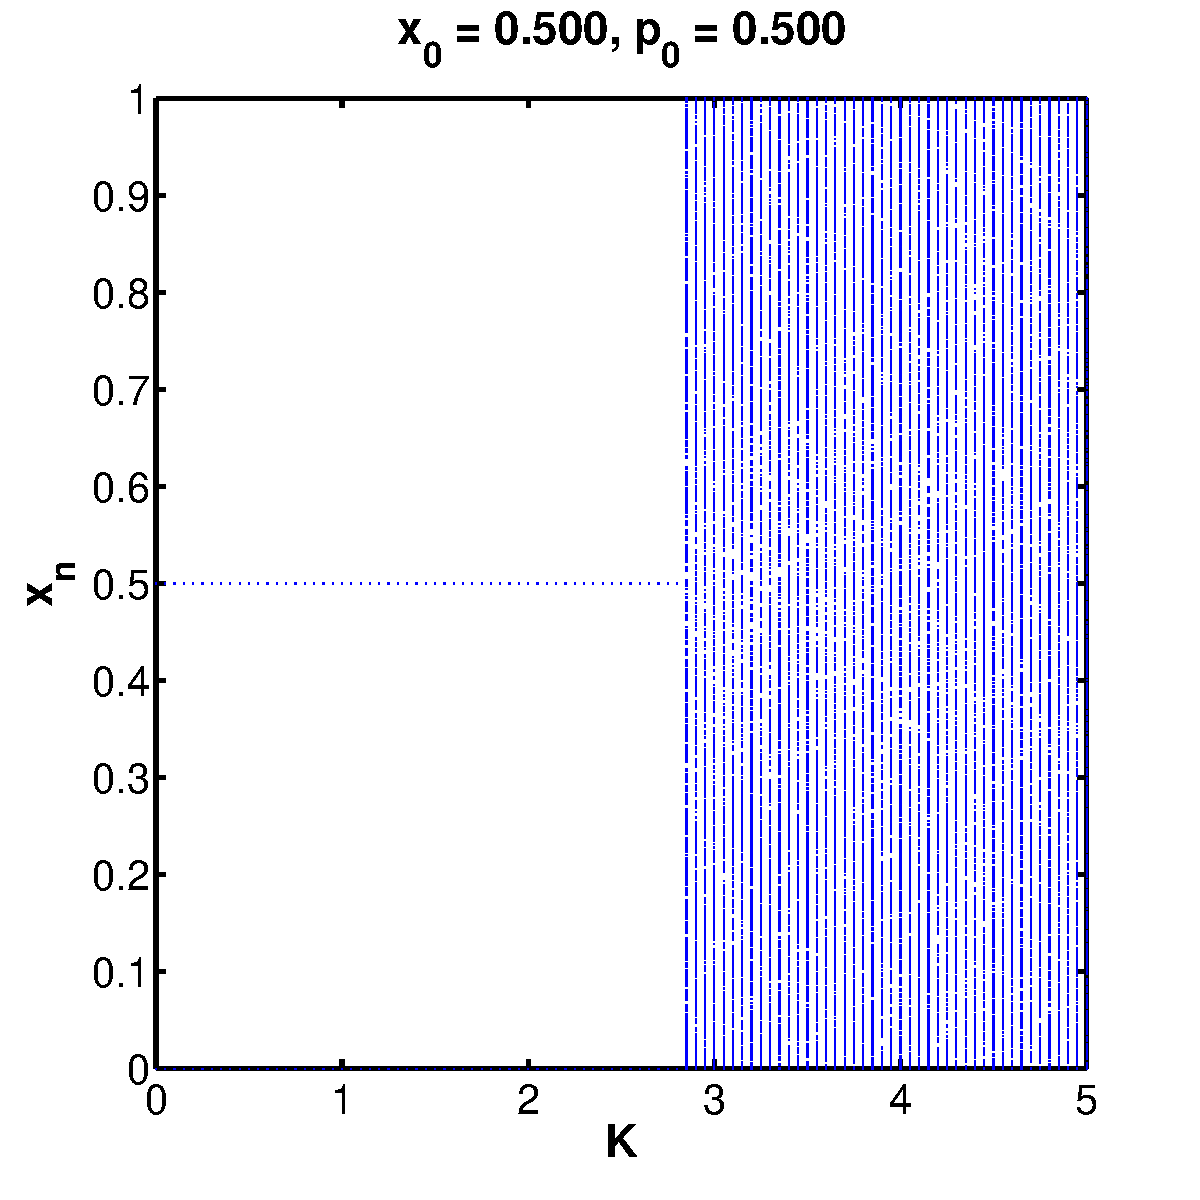
\includegraphics[width=\textwidth]{./img/assignment_b_dim_0_b_x}
			\caption{$x_0 = \num{0.234546}$}
			\label{fig:experiment:bifurcation:x}
	\end{subfigure}
	\begin{subfigure}{\columnwidth}
		\centering
			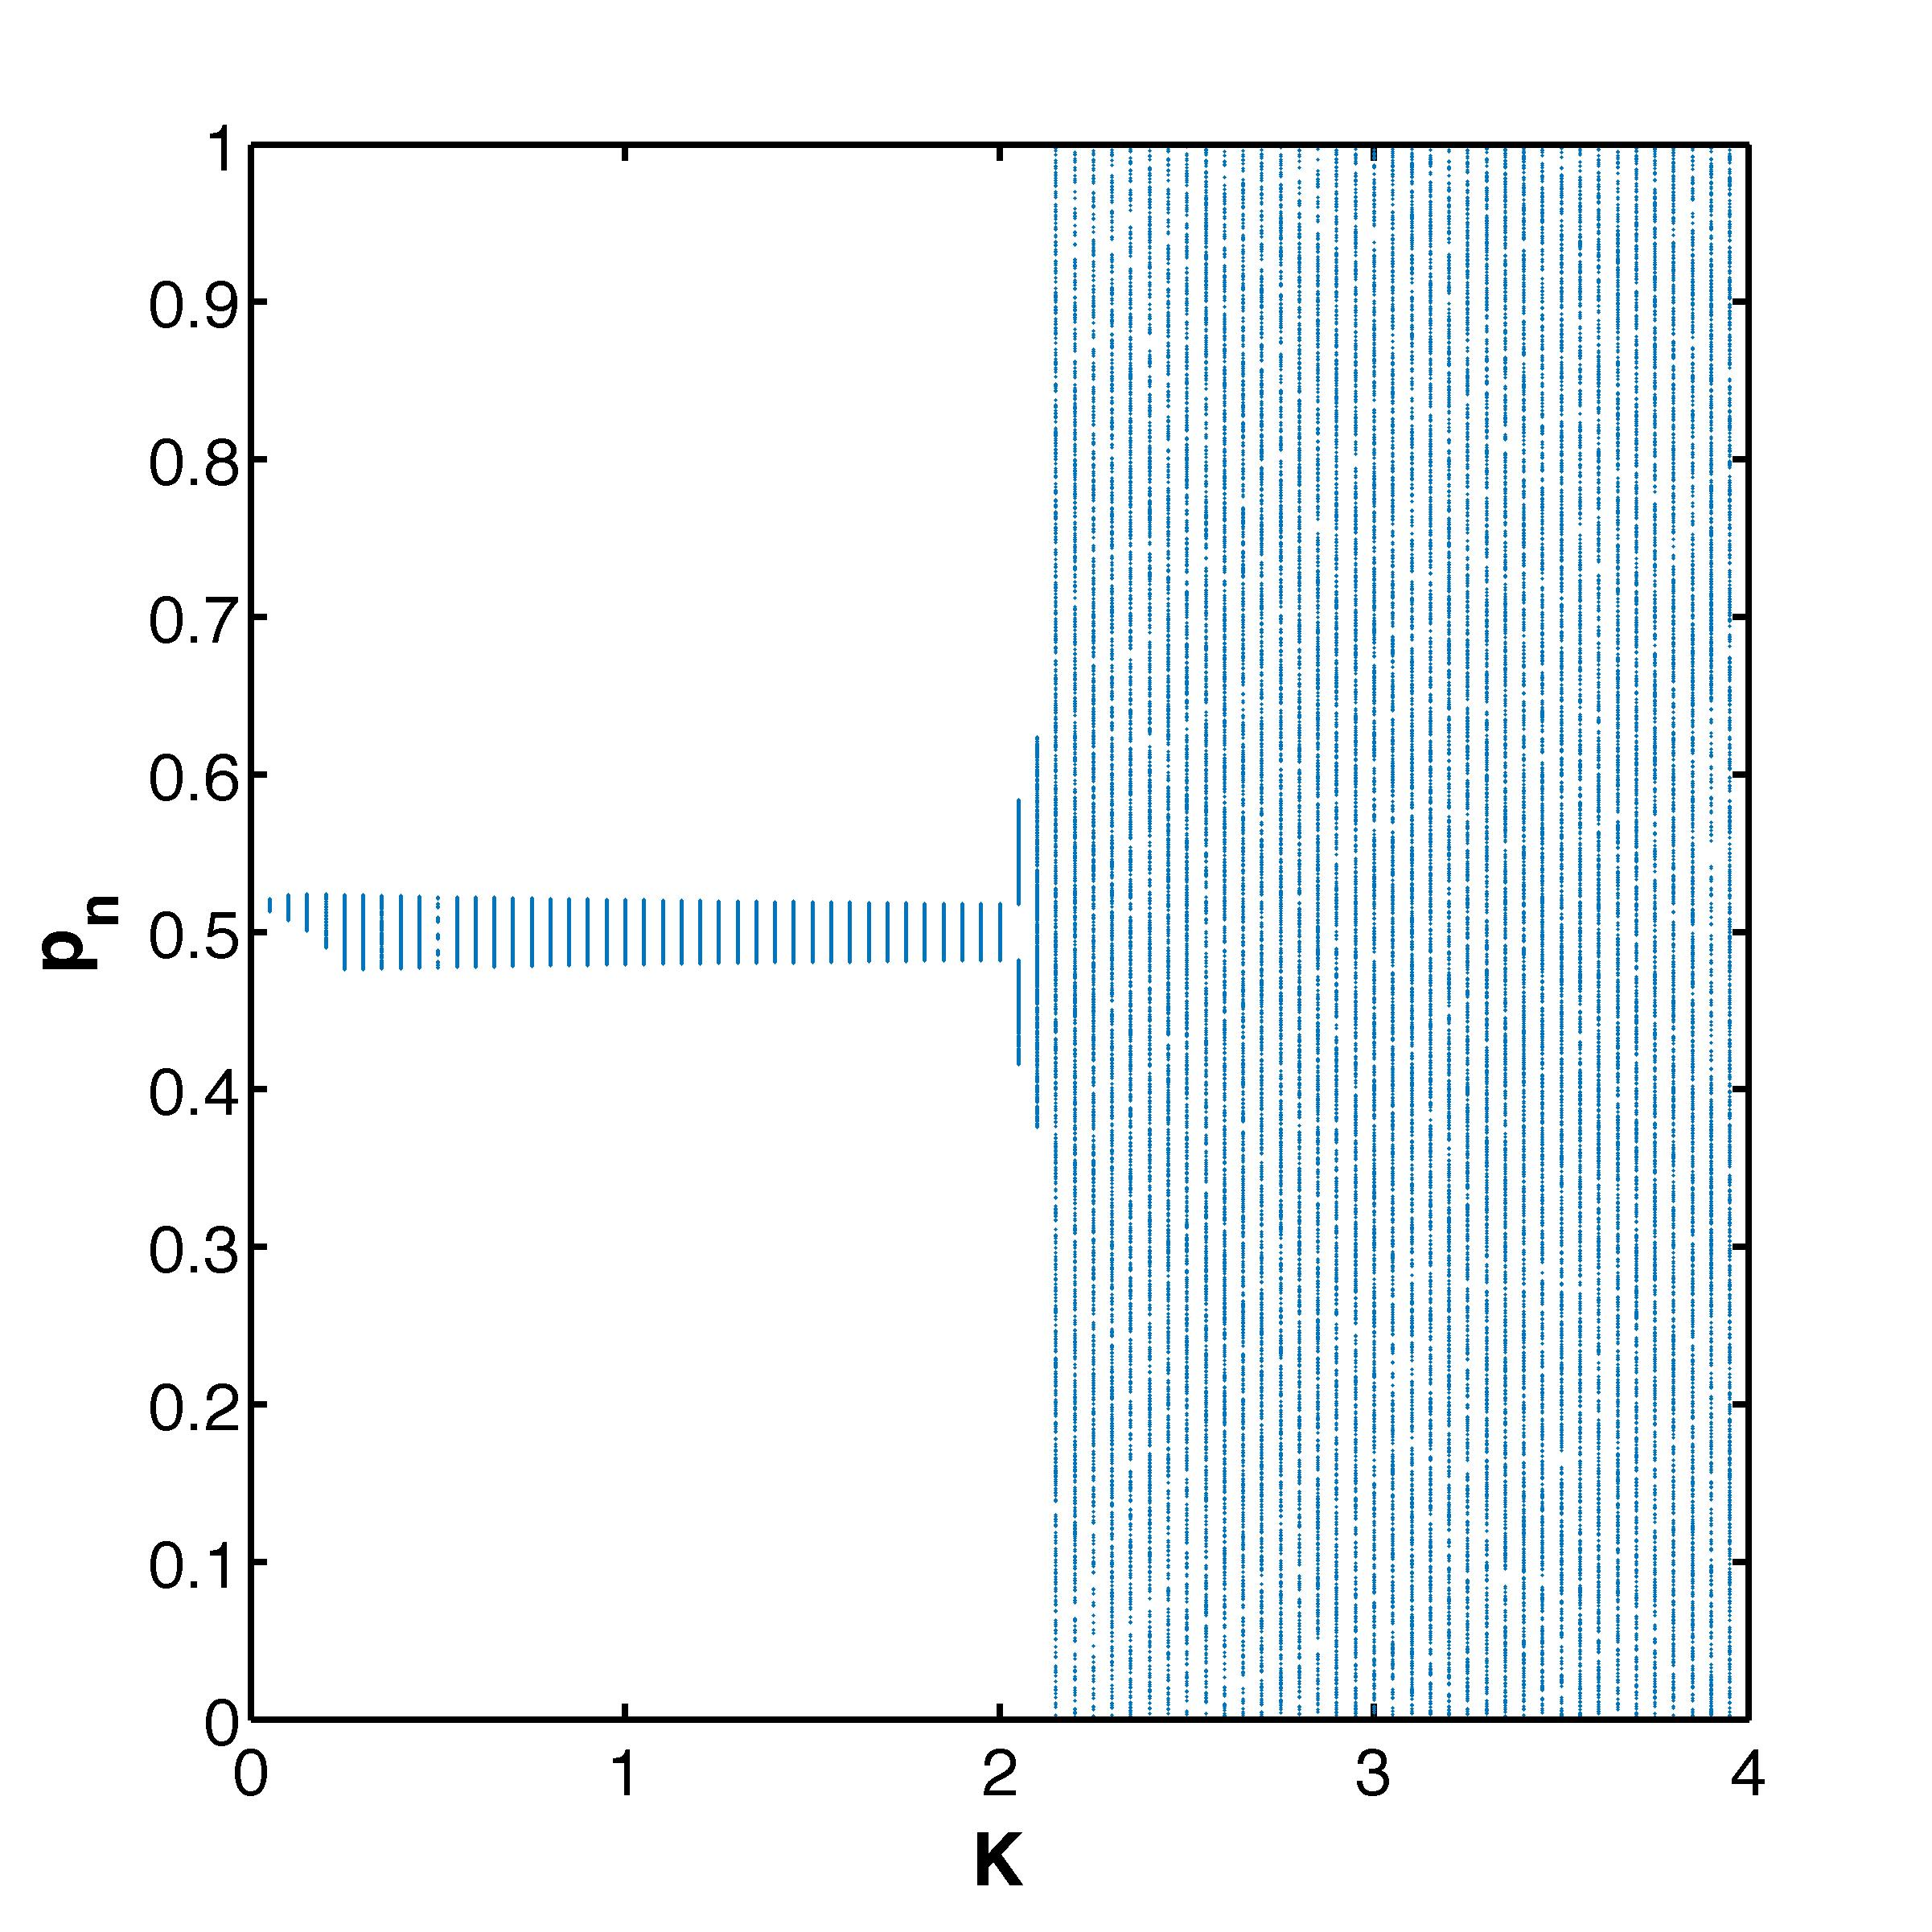
\includegraphics[width=\textwidth]{./img/assignment_b_dim_0_b_p}
			\caption{$p_0 = \num{0.112322}$}
			\label{fig:experiment:bifurcation:p}
	\end{subfigure}
	\caption{Bifurcation plot for $x_0 = \num{0.234546}$ and $p_0 = \num{0.112322}$ to illustrate the period doubling like effect in \cref{fig:experiment:fancy_k:2}}
	\label{fig:experiment:bifurcation}
\end{figure*}

\subsection{Non-Trivial Case}
\label{ss:b:nontrivial}
\todo[inline]{How do the orbits change with increasing K? Do we have scenarios that are similar to period doubling?}
\Cref{fig:experiment:fancy_k} shows the influence of the chaos driving variable $K$. All the images in \cref{fig:experiment:fancy_k} contain 100 Chirikov maps with randomly chosen values for $x_0$ and $p_0$. We consider a phase space to be more chaotic when there are more or bigger orbits (filled areas) in the images. \todo[inline]{Would be nice to find that $K_c$ value to be between $0.4$ and $0.8$...}

As can be expected from the discussion in our previous section the map created with $K = 0$ shows only horizontal filled or dotted lines \todo[inline]{Dotted lines: Period doubling?}. This results from the constant value for $p_n$ and periodic changing values for $x_n$. 

By increasing $K$ with relatively small steps $0.2$ up until one, see \cref{fig:experiment:fancy_k:2} - \ref{fig:experiment:fancy_k:40}, one can clearly see the influence of this variable. With a $K = 0.2$ we can see that the constant lines are replaced by the closed curves in the upper, lower, and centre part of the phase space. From a $K = 8$ we can see the creation of the first mentionable orbits i.e. the 2D regions start to grow in the upper and lower parts of the image in \cref{fig:experiment:fancy_k:8}. \todo[inline]{Which has probably something to do the KAM theory, I just found the $K_c$ value to be $0.618033$} Finally in the images shown in \cref{fig:experiment:fancy_k:20} - \ref{fig:experiment:fancy_k:40} we see that the orbits start to dominate, with in the last two images (\cref{fig:experiment:fancy_k:30} and \ref{fig:experiment:fancy_k:40}) only two stable points/areas/lines left. 



\todo[inline]{Discuss similarities and differences to logistic map}

\subsection{KAM-orbits}
\label{ss:b:kam}
\citeauthor{kenzel1997physics} define Kolmogorov-Arnold-Moser-orbits as one-dimensional orbits that traverse the entire phase-state diagram horizontally, in \cref{fig:experiment:fancy_k} they are represented by the solid lines. Looking closely at \cref{fig:experiment:fancy_k:0} we observe that not all orbits are $KAM$-orbits, since some of the lines are clearly dashed. An interesting property of the KAM-orbits is that it can be shown that chaotic orbits cannot cross the one-dimensional orbits \cite{kenzel1997physics}. Consequently they restrict the extent of the chaos of the two-dimensional orbits.\\

\begin{figure*}
	\centering
	\begin{subfigure}{\columnwidth}
		\centering
		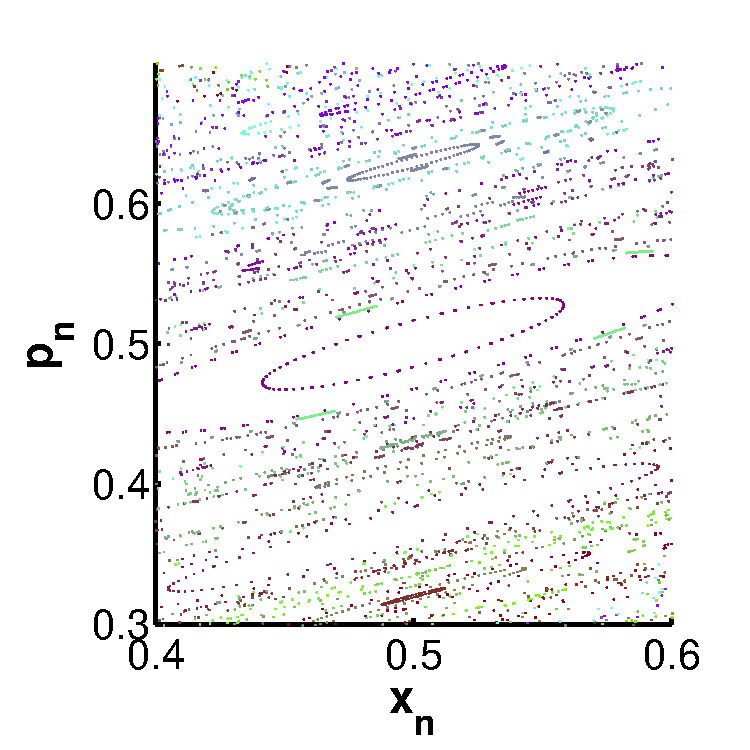
\includegraphics[width=\textwidth]{./img/assignment_b_fancy_k_9700}
		\caption{$K = 0.970000$}
		\label{fig:experiment:b:96}
	\end{subfigure}
	\begin{subfigure}{\columnwidth}
		\centering
		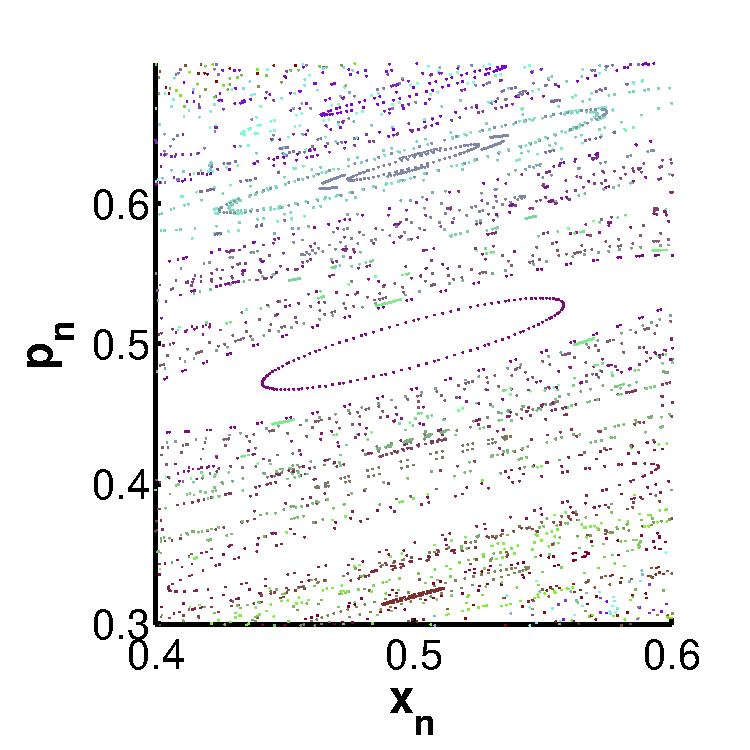
\includegraphics[width=\textwidth]{./img/assignment_b_fancy_k_9716}
		\caption{$K = K_c$}
		\label{fig:experiment:b:KC}
	\end{subfigure}	
	\caption{$p_n$ as a function of $x_n$ for $0.4 \leq x_n \leq 0.6$, $0 \leq p_n \leq 0.15$ and $0 \leq n \leq 250$. \subref{fig:experiment:b:96} show the phase-state diagram for $K = 0.970000$ and \subref{fig:experiment:b:KC} for $K + K_c$. The 200 initial values for $p$ and $x$ where chosen randomly, but were identical for both values of $K$.}
	\label{fig:experiment:b:testKC}
\end{figure*}

\citeauthor{greene1979method} observed that for small values of $K$ there are many KAM orbits that encircle the islands horizontally, see \cref{fig:experiment:fancy_k:0}, \ref{fig:experiment:fancy_k:2} and \ref{fig:experiment:fancy_k:4}. These KAM orbits divide the space into several compartments which may contain chaotic orbits. For larger values of $K$ there are fewer KAM orbits and individual chaotic orbits occur a greater are of the phase space. Finally at some critical value of $K$, called $K_c$, the last KAM orbit disappears, this effect can be observed in \cref{fig:experiment:fancy_k:10}. 

It has been found that for $K < K_c = 0.971635\dotsc$, one-dimensional-orbits exist that traverse the entire phase-state diagram horizontally \cite{kenzel1997physics}. If we plot the phase-state diagram for a value of $K$ that is slightly smaller than $K_c$, \cref{fig:experiment:b:96}, and for $K = K_c$, \cref{fig:experiment:b:KC}, we observe that the single KAM-orbit in \cref{fig:experiment:b:96} has disappeared in \cref{fig:experiment:b:KC}. 

